\begin{exercise}{Rendement de Curzon et Alhborn}{4}{Sup, spé}
{Thermodynamique, Machine thermique}{lelay,CurzonAhlborn1975}

\begin{questions}
    \questioncours Rappeler la forme du cycle de Carnot et démontrer la formule de l'efficacité de Carnot : $\eta = 1 -\frac{T_f}{T_c}$
    \question Est-il possible d'obtenir le rendement de Carnot avec une machine thermique réelle ? Que faut-il faire pour s'en approcher ? Quel problème pratique cela pose-t-il, au niveau de la puissance par exemple ?
\uplevel{En vue d'applications dans la vie réelle, on souhaite maintenant optimiser non pas l'efficacité mais la puissance de notre machine thermique.}    
    \question On considère un moteur de Carnot modifié tel que 
    \begin{enumerate}
        \item La détente isotherme à haute température se produit à température $T_1$ pendant un temps $t_1$, durant cette phase le moteur reste en contact avec le réservoir chaud à température $T_c > T_1$.
        \item La compression isotherme à basse température se produit à température $T_2$ pendant un temps $t_2$, durant cette phase le moteur reste en contact avec le réservoir foid à température $T_f < T_2$.
        \item Les phases adiabatiques sont très rapides, leur durée est négligeable.
    \end{enumerate}
    En utilisant le premier principe, calculer la puissance $W$ de ce moteur en fonction de $T_1$, $T_c$, $T_2$, $T_f$, $t_1$, $t_2$ et $C$.
    \question On pose $x = 1 - T_1/T_c$ et $y = T_2/T_f-1$. Quel est le signe de $x$ et de $y$ ? En utilisant le second principe, exprimer $\frac{t_1}{t_2}$ en fonction de $x$, $y$, $T_c$ et $T_f$.
    \question En remplaçant $\frac{t_1}{t_2}$ dans l'expression de la puissance, exprimer la puissance réduite $P' = P/C$ en fonction de $x$, $y$, $T_c$ et $T_f$.
    \question On cherche à maximiser la puissance de notre machine thermique. Comment exprimer cela mathématiquement ? 
    \question En se plaçant au point de puissance optimale, montrer que le rapport $\frac{y}{x}$ revêt une forme simple.
    \question Le rendement de cette machine thermique est $\eta' = 1-\frac{y}{x}\frac{T_f}{T_c}$. Discuter du rapport avec le rendement de Carnot.
    \question La table ci dessous est tirée de l'article original de Curzon et Ahlborn (1975). Calculer pour chaque centrale le rendement de Carnot et le rendement $\eta'$ de Curzon et Alhborn. Commenter.
\end{questions}

\begin{figure}[H]
    \centering
    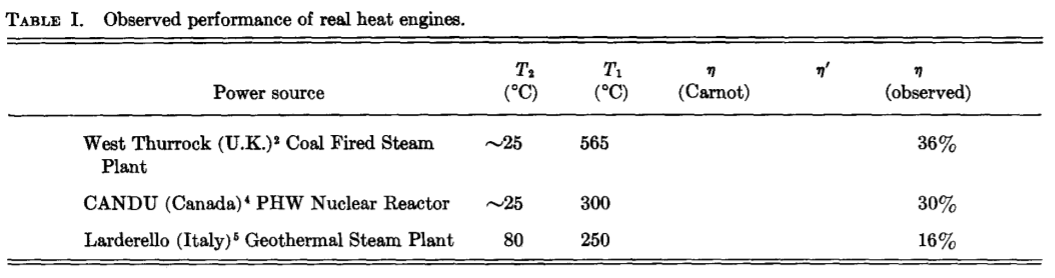
\includegraphics[width=0.9\textwidth]{thermo/machinesthermiques/RendementsCA.png}
    \caption{Table de rendements.}
\end{figure}

\end{exercise}

\begin{solution}
\begin{questions}
    \questioncours $\eta = 1 -\frac{T_f}{T_c}$
    \question Non, il faut attendre un temps infini : puissance nulle.
\uplevel{En vue d'applications dans la vie réelle, on souhaite maintenant optimiser non pas l'efficacité mais la puissance de notre machine thermique.}    
    \question Il faut traduire les données de l'énoncé
    \begin{enumerate}
        \item $Q_1 = C(T_c-T_1) t_1$.
        \item $Q_2 = C(T_2-T_f) t_2$.
        \item On reste sur un semi - moteur de Carnot, donc $\Delta S_{c} = 0$
    \end{enumerate}
    Le premier principe donne $W - Q_1 + Q_2 = 0$ et $P = \frac{W}{t_1+t_2}$, d'où
    \begin{align*}
        P = \frac{Q_1 - Q_2}{t_1+t_2} = \frac{C(T_c-T_1) t_1 - C(T_2-T_f) t_2}{t_1+t_2}
    \end{align*}
    L'EXO EST FAISABLE AVEC $C_1 \neq C_2$ IL EST JUSTE PLUS CHAUD.
    \question $x > 0$, $y > 0$, Le second principe donne $Q_1/T_1 = Q_2/T_2$ d'où 
    \begin{align*}
        \frac{t_1}{t_2} &= \frac{y}{x}\frac{1-x}{1+y}
    \end{align*}
    \question $P' = \frac{ xy\qty( (1-x)T_c ) - (1+y)T_f }{ x(1+y) + y(1-x) }$
    \question On veut $\pdv{P}{T_1} = \pdv{P}{T_2} = 0$ hence $\pdv{P'}{x} = \pdv{P'}{y} = 0$
    \question Les calculs sont violents, on trouve $\frac{y}{x} = \sqrt{\frac{T_c}{T_f}}$
    \question Pouit pouit la racine
\end{questions}
\end{solution}